% !TeX spellcheck = en_US

\section{Semantic Techniques}
\label{chapter:semantictechniques}

Figure~\ref{fig:ontology} depicts the hierarchical structure of my tourist inquiries ontology. It contains three main concepts, namely \textit{Category}, \textit{Location}, and \textit{Tourist Action}. As you can see I have neglected time and date dimensions present in the data warehouse model. I decided to develop this application in an iterative manner, starting from a simple model with a few concepts only, but with a complex hierarchical structure connecting them. Unfortunately, I did not had the time to integrate time/date later. Each concept pointed by an arrow is a super-class of the concept connected to it. 

\subsection{Classes}

The all-to-all connection pattern seen under Category is due to the fact, that the data source generated only 5 categories, where the \textit{Hotel} category is an umbrella term for \textit{Pension}, \textit{Garni}, \textit{Pub}, and \textit{Residence}. However, I thought of dividing these concepts, because the domain experts could separate them later on more easily. These concepts are defined as \textsc{Equivalent To} each other, and as \textsc{subclass of} Category. However, such details are not shown in the \textsc{OwlViz} graph.

The \textit{Location} hierarchy shows first the general concept of locations in the world, and then different granularities, such as \textit{Continent}, \textit{Country}, \textit{Province}, \textit{Touristic District}, and \textit{City or town}, where the latest one is defined as possible destination for tourists. In addition, I have defined a \textit{Ladin Town} as a \textit{City or town} with a ladin name.

The \textit{Tourist action} class contains currently only \textit{Inquiry} as subclass, which contains five defined classes \textit{Farm Inquiry}, \textit{Other Accommodation Inquiry}, \textit{Private Inquiry}, and a disjoint union of \textit{Inquiries for Hotel with 1-3 stars} and \textit{Inquiries for Hotels with 4-5 stars} composing a superclass \textit{Hotel Inquiries}.

\begin{figure}[h]
\centering
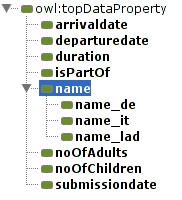
\includegraphics[width=0.3\linewidth]{img/data_property_hierarchy}
\caption{Data property hierarchy}
\label{fig:data_property_hierarchy}
\end{figure}

\begin{figure}[h]
\centering
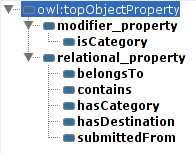
\includegraphics[width=0.3\linewidth]{img/object_property_hierarchy}
\caption{Object property hierarchy}
\label{fig:object_property_hierarchy}
\end{figure}

The inquiry class (referring to the inquiry fact table of the data warehouse) contains several data properties, such as \textit{name}, \textit{number of adults}, \textit{number of children}, \textit{date of submitting the inquiry}, \textit{arrival date}, \textit{departure date}, and \textit{duration of the holiday}. The whole hierarchy can be seen in Fig.~\ref{fig:class_inquiry_properties}. Each property is used exactly once for each inquiry, although some are defined as optional in the data warehouse design document. However, we can set it to a exact cardinality of one, because the value are always non-null (for instance, set to zero if numeric, and not defined). Finally, the \textit{name} properties are \textit{functional}.

\begin{figure}[h]
\centering
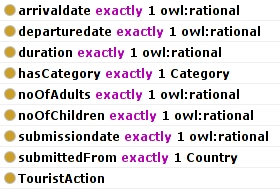
\includegraphics[width=0.4\linewidth]{img/class_inquiry_properties}
\caption{Inquiry data properties and constraints (modeled as \textsc{subclass~of} constraint)}
\label{fig:class_inquiry_properties}
\end{figure}

Subclasses of \textit{Inquiry} are defined as \textsc{Equivalent To} a class expression. For example, the \textit{Farm Inquiry} is equivalent to the following definition:
\begin{lstlisting}
Enquiry and (isCategory only Farm)
\end{lstlisting}
All other subclasses are defined analogous, except for \textit{Hotel Inquiry} which is a disjoint union of \textit{Hotel123Inquiry} and \textit{Hotel45Inquiry}, which are defined as follows
\begin{lstlisting}
HotelEnquiry and (isCategory only Hotel123)
HotelEnquiry and (isCategory only Hotel45)
\end{lstlisting}

\begin{sidewaysfigure}
	\centering
	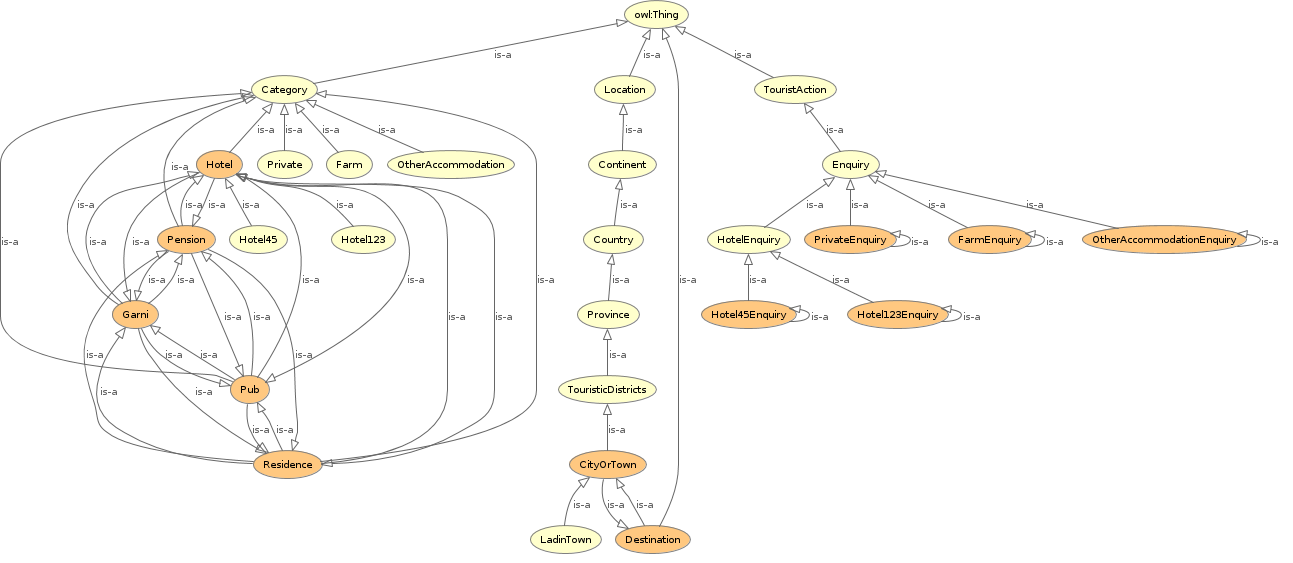
\includegraphics[width=\textwidth]{img/ontology.png}
	\caption{\textsc{OwlVIZ} representation of my tourist inquiries ontology}
	\label{fig:ontology}
\end{sidewaysfigure}




